\chapterimage{Mavrica.jpg} % Chapter heading image

\chapter{Detektorji svetlobe}

V tem poglavju bomo spoznali detektorje svetlobe, ki so nepogrešljivi
pri kvantitativni obravnavi optičnih pojavov. Detektorji se med seboj razlikujejo
po načinu delovanja in po svojih specifikacijah, ki jih bomo opisali v nadaljevanju. Največ
pozornosti bomo posvetili polprevodniškim detektorjem, ki so danes najbolj razširjeni.
Na koncu bomo spoznali še šum pri detekciji, ki omejuje uporabnost naprav.

\section{Osnovne karakteristike detektorjev}

Osnovna naloga optičnih detektorjev je pretvoriti vpadni svetlobni signal 
v nek drug signal, ki ga lahko natančno merimo. Navadno sta to električni tok 
ali električna napetost, ki sta sorazmerna z močjo vpadne svetlobe 
in ne z amplitudo električne poljske jakosti. V grobem delimo detektorje v dve skupini, 
na termične in kvantne. Prvi pretvorijo energijo vpadne svetlobe 
v toploto, drugi pa temeljijo na fotoefektu, kjer vpadli foton izbije elektron ali 
ustvari par elektron-vrzel.

Pri termičnih detektorjih zaznamo svetlobo tako,
da merimo povečanje temperature senzorja zaradi absorbirane svetlobe in taki detektorji
zaznavajo energijo vpadle svetlobe. Njihov odziv je razmeroma počasen, zato jih uporabljamo
predvsem za merjenje optične moči, lahko tudi zelo velike. Po drugi strani pa je odziv
termičnih detektorjev neodvisen
od valovne dolžine vpadne svetlobe, zaradi česar so termični detektorji uporabni na 
širokem območju od globoke ultravijolične do daljne infrardeče svetlobe. Uporaba
prevlada predvsem v infrardrečem, teraherčnem ali celo mikrovalovnem območju, kjer so 
drugi detektorji bistveno manj občutljivi. 
Primeri termičnih detektorjev so bolometer, termočlen in piroelektrični detektor.

Druga skupina so kvantni detektorji, v katerih se
fotoni absorbirajo in povzročijo pojav prostih nosilcev naboja. Taki detektorji
zaznavajo število vpadlih fotonov. Odlikuje jih zelo hiter odziv 
(tipično pod $\si{\micro\second}$)
in velika občutljivost. Njihova poglavitna slabost je omejen obseg valovnih dolžin,
pri katerih zaznavajo svetlobo, poleg tega jih je za optimalno delovanje treba 
hladiti. Primeri so vakuumske, polprevodniške in plazovne fotodiode.
\begin{figure}[h]
\centering
\def\svgwidth{65truemm} 
\input{slike/11_ShemaTermKv.pdf_tex}
\caption{Primerjava spektralnega odziva termičnega in kvantnega detektorja}
\label{fig:shemaTermKv}
\end{figure}

Osnovne karakteristike, ki omogočajo primerjavo med detektorji in določajo njihovo uporabnost,
so občutljivost, spektralni odziv, odzivni čas in prag detekcije. 

\begin{enumerate}
\item Občutljivost detektorja $R$ pove, koliko je izhodnega signala 
na enoto vpadnega svetlobnega toka. Enota za občutljivost je tako A/W ali V/W. 
\item Spektralni odziv pove, kako se občutljivost spreminja z valovno dolžino $R(\lambda)$.
Pri termičnih detektorjih je $R(\lambda)$ konstanta, medtem ko kvantni detektorji 
delujejo le v določenem območju valovnih dolžin, ki je odvisen od snovi, 
iz katere je detektor narejen. 
\item Odzivni čas pove, kako hitro se detektor odzove na spremembo optičnega signala. Predvsem 
optične telekomunikacije zahtevajo izredno hiter odziv.
\item Prag detekcije pove, pri kolikšni vpadni svetlobni moči postane razmerje med signalom ($S$)
in šumom ($N$, {\it noise}) enako $S/N = 1$. 
\end{enumerate}

\section{Termični detektorji}
Termične detektorje se zaradi njihovega razmeroma počasnega odziva uporablja predvsem 
za merjenje vpadne moči in za detekcijo svetlobe tistih valovnih dolžin, za katere 
ni drugih preprostih ali učinkovitih detektorjev. Pogosto se uporabljajo za termografske 
kamere in v astronomiji.

Delovanje termičnih detektorjev temelji na spremembi temperature zaradi absorpcije svetlobe 
(energije), detektorji pa se med seboj razlikujejo predvsem v načinu pretvorbe spremembe 
temperature v električni signal.
Tipalo termičnih detektorjev mora biti pri vseh vrstah dobro počrnjeno, da absorbira
svetlobo v čim širšem spektralnem območju. Čeprav je njihova občutljivost načeloma 
neodvisna od valovne dolžine vpadne svetlobe, se v praksi pojavijo omejitve zaradi
prepustnosti okna in absorpcijskega spektra črnega nanosa. Tipala so majhna, zato 
da dosežemo čim hitrejši odziv, ki pa je kljub temu navadno počasnejši od 1~ms. Sodobnejši
detektorji se po odzivnem času že približujejo kvantnim, saj dosegajo odzivne čase tudi do
$\sim 10~\si{\micro\second}$. Termične detektorje uporabljamo pri sobni temperaturi, 
za zahtevne meritve pa jih hladimo na nekaj K. 

Obravnavajmo termični detektor, katerega tipalo naj ima toplotno kapaciteto $C$. Toplota
se s tipala odvaja v nek toplotni rezervoar s temperaturo $T_0$, 
toplotne izgube pa označimo z $\Lambda$. Ko na tipalo vpada svetloba moč $P$, začne
temperatura tipala $T$ zaradi absorpcije svetlobe naraščati, hkrati pa se tipalo 
ohlaja zaradi odtekanja toplote:
\beq
\frac{dW}{dt} = C \frac{dT}{dt} = P - \Lambda (T-T_0).
\label{TD1}
\eeq
V stacionarnem stanju, ki ga dosežemo pri konstantnem vpadnem svetlobnem toku, se
temperatura tipala ne spreminja in razlika temperature tipala in rezervoarja je 
\beq
T - T_0 = \frac{P}{\Lambda}.
\label{temp_sens}
\eeq
Občutljivost detektorja, ki je sorazmerna z razliko temperatur, 
je torej obratno sorazmerna s toplotnimi izgubami. Za večjo občutljivost moramo
torej toplotne izgube detektorja kar se da zmanjšati. 

Po enačbi~(\ref{TD1}) se temperatura približuje stacionarni vrednosti s časovno konstanto 
\beq
\tau = \frac{C}{\Lambda},
\label{TermD_t}
\eeq
ki je ključni parameter za določanje odzivnega časa detektorja. Odzivni
čas je sorazmeren s kapaciteto senzorja, zato so tipala praviloma zelo majhna.
Vidimo, da moramo za dosego čim krajšega odzivnega časa toplotne izgube kar se da povečati. Če velike
izgube skrajšajo odzivni čas, pa po drugi strani zmanjšajo občutljivost (enačba~\ref{temp_sens}), 
zato pri termičnih detektorjih ne moremo imeti hkrati velikega in hitrega odziva. 
Če želimo toplotne izgube povečati, da s tem skrajšamo odzivni čas, detektorje hladimo z zrakom 
ali celo z vodo, majhne toplotne izgube pa so omejene s sevanjem.  

Podrobneje poglejmo odziv termičnega detektorja od vpadne moči. Naj se vpadna moč
spreminja s časom, temperatura na detektorju pa temu sledi z določeno zakasnitvijo. Odziv
najlepše izračunamo v Fourierevem prostoru. Vpadno moč in temperaturo izrazimo kot
\beq
P(t) = \int_{-\infty}^{\infty} P_\omega e^{i\omega t}d\omega \quad \mathrm{in} \quad
T = T_0 + \int_{-\infty}^{\infty} T_\omega e^{i\omega t}d\omega.
\label{TermTF}
\eeq
To vstavimo v enačbo~(\ref{TD1}) in dobimo
\beq
\int_{-\infty}^{\infty} i \omega T_\omega e^{i\omega t}d\omega = \frac{1}{C}
\int_{-\infty}^{\infty} (P_\omega - \Lambda T_\omega) e^{i\omega t}d\omega.
\eeq
Enačbi zadostimo, če izenačimo člene pred vsako spektralno komponento posebej
\beq
i \omega T_\omega = \frac{1}{C}\left(P_\omega - \Lambda T_\omega\right).
\eeq
Če vpeljemo odzivni čas $\tau$ (enačba~\ref{TermD_t}), sledi
\beq
T_\omega = \frac{1}{\Lambda}\left(\frac{1}{1+i \omega \tau}\right)P_\omega.
\label{TermOdziv}
\eeq

\begin{definition}
Pokaži, da je odziv termičnega detektorja na zelo kratek svetlobni sunek oblike 
$P(t) = P_0 \delta(t-t_0)$ enak 
\beq
T(t)=\frac{iP_0}{\Lambda}e^{-(t-t_0)/\tau}.
\eeq
\end{definition}

\subsection*{Bolometer}
Bolometer je termični detektor, pri katerem zaznavamo spremembo električne upornosti
zaradi spremembe temperature tipala\footnote{Prvi bolometer je leta 1881 naredil
ameriški fizik, astronom in letalski inženir Samuel Pierpont Langley, 1834--1906.}. 
Tipalo je praviloma počrnjena tanka ploščica, 
navadno je narejena iz termistorja, polprevodnika ali superprevodnika. Tipalo preko
referenčnega upora priključimo na napetost, preko kondenzatorja pa merimo napetost na njem.
Za meritve konstantega svetlobnega toka tipalo navadno vežemo v Wheatstonov mostiček. V obeh
primerih za referenčni upor vzamemo kar enako tipalo, ki ga zaščitimo pred vpadno svetlobo, 
tako da postane sistem neobčutljiv na morebitne spremembe temperature okolice.
\begin{figure}[h!]
\centering
\def\svgwidth{90truemm} 
\input{slike/11_bolometer.pdf_tex}
\caption{Shema bolometra}
\label{fig:Bolometer-shema}
\end{figure}

Prednost bolometrov s termistorjem je približno linearna zveza med upornostjo in 
temperaturo. Uporabljamo jih predvsem za merjenje večjih vpadnih moči, saj taki 
detektorji niso zelo občutljivi ($R\sim 100~\si{\volt/\watt}$). 
So pa robustni, stabilni in delujejo pri sobni 
temperaturi. Odzivni časi so okoli $\tau \sim 1$--$20~\si{\milli\second}$. 
Pri polprevodniških bolometrih upornost pojema eksponentno s temperaturo. 
Primerni so za detekcijo teraherčnih valovanj, vendar mora biti za ta namen 
bolometer (npr. germanijev) hlajen s tekočim helijem. Tako lahko dosežemo
občutljivosti večje od $R \sim 10^8~\si{\volt/\watt}$. Zelo občutljivi so tudi 
detektorji s superprevodnimi tipali, saj je odvisnost upornosti od temperature v bližini
prehoda v superprevodno stanje zelo velika ($R \sim 10^3~\si{\volt/\watt}$).

\begin{figure}[h]
\centering
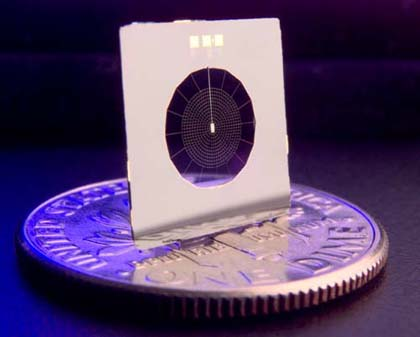
\includegraphics[width=80truemm]{slike/11_Bolometer.jpg}
\caption{Bolometer za merjenje prasevanja. Premer kovanca za primerjavo je 18~mm. 
Vir: NASA/JPL-Caltech.}
\label{fig:Bolometer}
\end{figure}

\subsection*{Termočlen}
Termočlen je sestavljen iz dveh različnih vodnikov. En spoj vodnikov počrnimo, drugega, 
referenčnega, pa zaščitimo pred svetlobo. Zaradi vpadne svetlobe se počrnjeni spoj 
segreje, med obema spojema nastane temperaturna razlika in zaradi termoelektričnega 
pojava tudi električna napetost, ki jo lahko merimo. Pri tem pazimo, da je prevodnost
vodnikov čim večja, toplotna prevodnost pa čim manjša. Odzivni čas termočlenov je 
okoli $\tau \sim 10$--$20~\si{\milli\second}$, občutljivost pa okoli $R \sim 10~\si{\volt/\watt}$.
Ker so napetosti, ki se pojavijo med stikoma, razmeroma majhne (le okoli 
$\sim 10~\si{\micro\volt/K}$) pogosto vežemo več (nekaj deset) termočlenov zaporedno v
termobaterijo. Občutljivost s tem naraste na $R \sim 200~\si{\volt/\watt}$, podaljša 
pa se časovna konstanta $\tau \sim 10$--$2000~\si{\milli\second}$. Prednost termočlenov je,
da za svoje delovanje ne potrebujejo zunanjega napajanja. 

\subsection*{Piroelektrični detektor}
Piroelektriki so snovi brez centra inverzije, v katerih je lastna električna 
polarizacija odvisna od temperature (npr. LiTaO$_3$, triglicin sulfat TGS 
in vsi feroelektriki). Piroelektrični detektor je narejen iz 
ploščice piroelektrične snovi med dvema elektrodama oziroma ploščama kondenzatorja.
Ko se ploščica zaradi absorbirane svetlobe segreje, se ji spremeni polarizacija in 
med elektrodama se pojavi premikalni tok, ki ga merimo na merilnem uporniku.

Zveza med spremembo temperature in spremembo polarizacije je
\beq
dP = a dT,
\eeq
kjer je $a$ piroelektrični koeficient. 

Med obema elektrodama s površino $S$ preteče naboj
\beq
de = I dt = S dP = S a dT.
\eeq
Tok skozi tipalo je tako
\beq
I = S a \frac{dT}{dt}.
\label{piro}
\eeq
Piroelektrični detektor je torej občutljiv na časovni odvod temperature detektorja, 
s tem pa tudi na spreminjanje vpadne svetlobne moči. V stacionarnem stanju 
detektor ne proizvaja električnega toka, zato moramo za merjenje 
konstantnega svetlobnega toka vpadno svetlobo najprej modulirati.
Navadno to naredimo kar z mehanskim zaklopom. Piroelektrični detektorji
se večinoma uporabljajo kot preprosti infrardeči detektorji. 
Njihova občutljivost je $R \sim 1~\si{\micro\ampere/\watt}$, odzivni čas pa odvisen od 
upornika v vezju, ampak lahko doseže vrednosti $\tau \sim 10~\si{\micro\second}$.

Poglejmo temperaturni odziv na tipalu. Izhajamo iz enačb~(\ref{TermTF}), (\ref{TermOdziv}) in
(\ref{piro}) in izračunajmo tok $I$ v odvisnosti od frekvence modulacije.
\beq
I = Sa \frac{dT}{dt} = Sa \frac{d}{dt} \int_{-\infty}^{\infty} T_\omega e^{i\omega t}d\omega 
=Sa\int_{-\infty}^{\infty}\frac{1}{\Lambda}\left(\frac{P_\omega}{1+i \omega \tau}\right) \,i \omega\,
e^{i\omega t}d\omega.
\eeq
Sledi 
\beq
I_\omega = \frac{i \omega\, SaP_\omega/\Lambda}{1 + i \omega \tau}.
\eeq
Vidimo, da pri majhnih frekvencah tok narašča, pri velikih frekvencah pa postane neodvisen od
frekvence modulacije vpadne svetlobe. Vendar to še ne pomeni, da lahko moduliramo s poljubno 
veliko frekvenco. Poleg relaksacijskega časa detektorja ima namreč karakteristični čas tudi
elektronsko vezje, ki določa zgornjo mejo za frekvenco. Ta je enak $\tau_e = R_eC_e$, pri čemer
sta $R_e$ upornost sistema in $C_e$ električna kapaciteta detektorja. 
\begin{figure}[h]
\centering
\def\svgwidth{65truemm} 
\input{slike/11_Piro.pdf_tex}
\caption{Spektralni odziv piroelektričnega detektorja na eni strani določajo toplotne izgube 
$\Lambda$ in toplotna kapaciteta detektorja $C$, navzgor pa odziv omejuje odziv elektronskega vezja $\tau_e$.}
\label{fig:Piro}
\end{figure}

\begin{definition}
Piroelektrični detektor naredimo iz kristala LiTaO$_3$ s koeficientom piroelektričnosti
$a = 2,3 \times 10^{-4}~\si{\ampere \second /\metre^2 \kelvin}$ in povprečno 
dielektričnostjo $\varepsilon = 50$. Izračunaj dovoljeno električno upornost sistema, 
če želimo, da detektor deluje za frekvence do 1~MHz. 
Dimenzija detektorja je $S = 1~\si{\centi\metre^2}$ in debelina $d = 1~\si{\milli\metre}$.
\end{definition}

\section{Fotoefekt}
Delovanje kvantnih detektorjev temelji na fotoefektu. To je pojav, pri katerem vpadli
fotoni iz snovi izbijajo elektrone. Izbiti elektroni lahko ubežijo kot prosti elektroni
(t. i. zunanji fotoefekt), ali pa ostanejo ujeti v snovi -- a mobilni -- in tako povečajo 
njeno prevodnost (notranji fotoefekt). V obeh primerih pride do fotoefekta le, 
če je energija vpadlih fotonov večja od neke določene energije.
Pod to vrednostjo fotoefekta ni, ne glede na moč vpadne svetlobe.
Fotoefekt je prvič opazil Hertz\footnote{Nemški fizik Heinrich Hertz, 1857--1894.} 
leta 1887, za njegovo razlago leta
1905 pa je Einstein\footnote{Nemški fizik in nobelovec Albert Einstein, 1879--1955.} 
dobil nobelovo nagrado. 

Poglejmo najprej zunanji fotoefekt, pri katerem elektron postane povsem prost. 
Da se to sploh lahko zgodi, mora biti energija vpadlega fotona dovolj velika, da 
elektron premaga potencialno bariero in izstopi iz prevodnega pasu (slika~\ref{fig:Nivoji}\,a). 
Najmanjšo energijo, ki je za to potrebna, imenujemo v kovinah izstopno delo. 
Če je energija fotona večja, gre preostanek energije v kinetično energijo izbitega
elektrona.

\begin{figure}[h]
\centering
\def\svgwidth{140truemm} 
\input{slike/11_Nivoji.pdf_tex}
\caption{Shema energijskih pasov in zunanjega fotoefekta v kovini (a) in polprevodniku (b) ter
notranjega fotoefekta v polprevodniku (c). $\Phi$ označuje izstopno delo, $E_g$ širino reže 
med valenčnim in prevodnim pasom poprevodnika,
$E_a$ pa elektronsko afiniteto. }
\label{fig:Nivoji}
\end{figure}

Zunanji fotoefekt poteka tudi v polprevodnikih (slika~\ref{fig:Nivoji}\,b). 
V tem primeru foton izbije elektron iz valenčnega pasu, njegova energija pa mora biti 
večja od vsote energije reže in elektronske afinitete, da lahko elektron zapusti snov. 
Z uporabo ustreznih materialov lahko dosežemo, da je elektronska afiniteta
negativna in je zato potrebna energija fotona kar enaka širini energijske reže.

Izstopno delo za kovine $\Phi$ je od okoli 2~eV za cezij pa do okoli 6~eV za platino. 
Ustrezna valovna dolžina svetlobe, ki še povzroči fotoefekt, je tako 
\beq
\lambda \leq \frac{hc}{\Phi},
\eeq
kar je 580~nm za primer cezija in samo okoli 200~nm za platino. Če želimo fotoefekt
izkostisti za detektorje vidne svetlobe, uporabimo druge snovi,
na primer Cs-Te, Cs-Sb, Na-K-Sb-Cs ali GaAs:Cs. 
Tako lahko zaznavamo fotone z valovnimi dolžinami od ultravijolične svetlobe 
pa vse do bližnje infrardeče. 

Pri notranjem fotoefektu (slika~\ref{fig:Nivoji}\,c) elektron snovi ne zapusti, ampak zgolj preide iz enega 
energijskega pasu v drugega. Tipično to poteka v polprevodnikih, kjer absorpcija fotona 
povzroči nastanek para elektron-vrzel, prag za nastanek para pa določa širina reže med 
energijskima nivojema. Primeri detektorjev, ki temeljijo na zunanjem fotoefektu, so 
fotocelice in fotopomnoževalke, na notranjem fotoefektu pa temeljijo na primer
fotoprevodniki, polprevodniške in plazovne fotodiode.

Za zdaj smo napisali, da fotoefekt poteče, ko foton izbije elektron. Vendar pri tem ni 
uspešen prav vsak foton, zato vpeljemo še en parameter, ki ga imenujemo kvantni izkoristek $\eta$.
Ta parameter pove verjetnost, da vpadli foton z valovno dolžino $\lambda$ oziroma frekvenco $\nu$ iz 
snovi izbije elektron. Električni tok, ki steče pri vpadni svetlobni moči $P$, je tako
\boxeq{11:eta}{
I = \eta e_0 N_F = \eta \frac{e_0 P}{h \nu},
}
kje je $N_F$ število vpadnih fotonov na časovno enoto.
Kvantni izkoristek je močno odvisen od valovne dolžine vpadne svetlobe in seveda
od snovi, na katero svetloba vpada. Za fotone z energijo, ki je manjša od izstopnega 
dela oziroma od širine energijske reže, je kvatni izkoristek praktično enak nič, 
nato pa strmo naraste in lahko doseže vrednosti, večje od $90~\%$. Podrobneje ga bomo 
obravnavali pri posameznih primerih detektorjev.

\begin{remark}
V praksi ločimo dve vrsti kvantega izkoristka: zunanji in notranji. Zunanji je vpeljan kot 
razmerje števila izbitih elektronov in fotonov, ki vpadejo na detektor. Ker pa se 
ob vpadu na detektor vedno nekaj fotonov odbije ali siplje, vpeljemo še notranji kvatni 
izkoristek kot razmerje števila elektronov in fotonov, ki se dejansko absorbirajo v detektorju.
Zunanji izkoristek je vedno manjši od notranjega in je neke vrste efektivni izkoristek.
\end{remark}

Iz enačbe(\ref{11:eta}) hitro izračunamo še občutljivost detektorja 
\boxeq{11:R}{
R = \frac{I}{P} = \frac{\eta e_0 }{h \nu}.
}

\section{Vakuumska fotodioda (fotocelica) in fotopomnoževalka}
\subsection*{Fotocelica}
Najpreprostejši kvantni detektor na zunanji fotoefekt je fotocelica ali vakuumska fotodioda
(slika~\ref{fig:Fotoefekt}). Fotocelica deluje tako, da svetloba vpada na katodo, 
zaprto v vakuumirani stekleni bučki, in tam povzroči fotoefekt. Izbite elektrone 
z zunanjo napetostjo pospešimo do anode in merimo električni tok, ki steče med 
katodo in anodo. Ker je tok sorazmeren s številom vpadlih fotonov, lahko na ta 
način izmerimo moč vpadne svetlobe.

\begin{figure}[h]
\centering
\def\svgwidth{60truemm} 
\input{slike/11_Fotoefekt.pdf_tex}
\caption{Shema fotocelice, v kateri poteka fotoefekt. 
Vpadna svetloba iz kovinske katode izbije elektrone, zaradi česar med katodo 
in anodo steče tok.}
\label{fig:Fotoefekt}
\end{figure}

Območje detekcije fotocelice je določeno z izstopnim delom kovine, iz katere fotoni izbijajo elektrone. 
Potrebno energijo fotona lahko precej zmanjšamo, če namesto čistih kovin uporabimo bi- ali 
večalkalne katode (npr. Na$_2$KSbCs), ali pa polprevodnike, na katere nanesemo tanko plast 
Cs ali Cs$_2$O. Tako ustvarimo negativno elektronsko afiniteto in izstopno delo je enako širini energijske
reže. Na ta način lahko zaznavamo svetlobo do valovnih dolžin okoli $1600~\si{\nano\metre}$. 
Na ultravijoličnem območju je delovanje
omejeno na okoli $160~\si{\nano\metre}$ zaradi neprepustnosti stekla, iz katerega je narejena bučka.
\begin{figure}[h]
\centering
\def\svgwidth{130truemm} 
\input{slike/11_SpekterKatode.pdf_tex}
\caption{Kvantni izkoristek fotocelic za različne snovi. Povzeto po Hamamatsu Photonics.}
\label{fig:Fotodioda}
\end{figure}

Čas odziva vakuumske fotodiode je odvisen od časa preleta elektronov od katode do anode. 
Da je ta čas čim krajši, je napetost na fotocelici pogosto več kV. Tedaj lahko dosežemo 
zelo kratke odzivne čase, tudi do 0,1~ns. Enostavnost in hitrost sta torej prednosti fotocelice, 
njena glavna pomanjkljivost pa je razmeroma nizek kvantni izkoristek. 
Ta je seveda močno odvisen od valovne dolžine vpadlega valovanja in snovi, iz 
katere je narejena katoda. Največje vrednosti, ki jih dosega, so okoli $40~\%$, 
pogosto pa več velikostnih redov manj. 
Vrednosti so razmeroma nizke, saj se izbiti elektroni gibljejo v vse
smeri in se pogosto sipljejo, preden sploh dosežejo površino. 

Dodaten problem fotocelic je, da pri končnih temperaturah prihaja do spontane oddaje elektrona.
Nekaj električnega toka zato teče tudi v popolni temi. To je rako imenovani temni 
tok fotodiode in tipično dosega vrednosti okoli $10^{-15}~\si{\ampere}$, lahko pa tudi do več nA. 
Za občutljive meritve je treba zato vakuumsko fotodiodo hladiti. 

\vskip1cm
\begin{definition}
Izračunaj občutljivost fotocelice na osnovi GaAs za valovanje z valovno dolžino $\lambda=620$~nm.
Pri tem kvantni izkoristek odčitaj s slike~(\ref{fig:Fotodioda}).
\end{definition}

\subsection*{Fotopomnoževalka}
Fotopomnoževalke so fotocelice z vgrajenim ojačanjem. Ojačanje dosežemo tako, da 
izbit fotoelektron najprej pospešimo z napetostjo $100$--$150~\si{\volt}$ na vmesno elektrodo, 
tako imenovano dinodo, iz katere izbije več ($\sim 5$--$10$, redkeje tudi do 40) 
sekundarnih elektronov. Ti elektroni
potujejo do naslednje dinode, ki je pod višjo pozitivno napetostjo (tipično okoli $100~\si{\volt}$
višjo), kjer ponovno izbijejo elektrone, ki vpadejo na naslednjo dinodo, ki je pod še višjo napetostjo ... 
To pomnoževanje se večkrat ponovi (navadno okoli desetkrat),
število elektronov eksponentno narašča in na en vpadli foton lahko dobimo $10^9$ elektronov na anodi. 
Občutljivost fotopomnoževalk je tako precej večja od občutljivosti vakuumske fotodiode in
dosega odzivnost na anodi do $R\sim 10^6~\si{\ampere/\watt}$.
Fotopomnoževalka tako omogoča štetje posameznih fotonov, po drugi strani pa moramo pri 
običajnih osvetlitvah paziti, da fotopomnoževalke ne osvetlimo preveč. 
\begin{figure}[h]
\centering
\def\svgwidth{80truemm} 
\input{slike/11_PMT.pdf_tex}
\caption{Shema fotopomnoževalke. Vpadna svetloba iz katode izbije elektrone, ti pa 
iz dinod izbijajo dodatne elektrone in izhodni signal se močno ojača.}
\label{fig:PMT}
\end{figure}

Fotopomnoževalke imajo zelo kratek odzivni čas, ki je odvisen od postavitve dinod. Posamezni 
elektroni do anode potujejo različno dolgo, zato je sunek na izhodu 
razširjen, tipično okoli $\sim 0,1$--$20~\si{\nano\second}$.  
Za manj zahtevne aplikacije pogosto merimo kar povprečni tok z anode. Kadar pa opazujemo
posamezne fotone, zaznamo na izhodu zaporedje sunkov. Takrat lahko 
amplituda izhodnega signala močno niha, saj je koeficient ojačanja 
odvisen od števila izbitih elektronov, kar pa je statistični proces. 

\section{Fotoprevodni detektorji}
Fotoprevodni detektorji\footnote{Fotoprevodne detektorje včasih imenujejo tudi fotouporniki.} 
so detektorji, ki temeljijo na notranjem fotoefektu.
Vpadli foton z dovolj veliko energijo se absorbira, vendar ne izbije elektrona v prostor, 
ampak ga iz valenčnega pasu dvigne v prevodnega. Pri tem nastane par elektron-vrzel. 
Ob priključeni napetosti se ti nosilci naboja začnejo premikati in steče tok, 
ki ga merimo. Z naraščajočim številom fotonov se prevodnost fotoprevodnika veča, 
zato lahko z merjenjem upornosti določimo 
intenziteto vpadle svetlobe. Tipično so fotoprevodniki iz polprevodnikov, 
lahko pa so tudi iz izolatorjev. 

Da foton lahko vzbudi elektron iz valenčnega v prevodni pas, mora biti njegova energija dovolj velika. 
V čistih (nedopiranih) polprevodnikih to pomeni, da mora biti energija fotona večja od 
širine reže. Za silicij, na primer, je širina reže 1,1~eV, s čimer lahko zaznavamo svetlobo
z valovno dolžino do okoli 
$1,1~\si{\micro\meter}$, za germanij 0,67~eV ($1,8~\si{\micro\meter}$) in za PbS 0,37~eV
($3,4~\si{\micro\meter}$). Za detekcijo daljših valovnih dolžin ne uporabljamo polprevodnikov
z manjšo energijsko režo, ampak dopirane polprevodnike (slika~\ref{fig:FPrevodnik}). 
Z novim energijskim nivojem med valenčnim in prevodnim pasom občutno zmanjšamo 
potrebno energijo vpadlih fotonov. Vendar je pri teh nizkih energijah prispevek termično 
vzbujenih elektronov že tako velik, da je treba detektorje hladiti, navadno s tekočim
dušikom ali celo tekočim helijem. Tak primer je germanij, dopiran s cinkom, 
s katerim lahko zaznavamo svetlobo do okoli $40~\si{\micro\meter}$. Pri tem ga hladimo
na $4~\si{\kelvin}$, da zmanjšamo pojav termično vzbujenih nosilcev naboja. 
\begin{figure}[h]
\centering
\def\svgwidth{150truemm} 
\input{slike/11_FPrevodnik.pdf_tex}
\caption{Shema prehoda elektrona v fotoprevodniku: prehod v čistem polprevodiku (a), 
$n$-dopiranem polprevodniku (b) in $p$-dopiranem polprevodniku (c). 
Z dopiranjem povečamo območje delovanja detektorja v infrardeče območje. }
\label{fig:FPrevodnik}
\end{figure}

Izračunajmo električni tok, ki steče, ko posvetimo na fotoprevodnik. Spomnimo se, da
je gostota električnega toka $j$ enaka vsoti prispevkov elektronov in vrzeli
\beq
j = e_0 n_v v_v + e_0 n_e v_e,
\eeq
pri čemer $n_v$ in $n_e$ pomenita gostoto vrzeli in elektronov v snovi, $v_v$ in $v_e$ pa 
hitrost vrzeli in elektronov. Ta je sorazmerna z električno poljsko jakostjo $E$, ki je priključena
 na vzorec, sorazmernostni faktor pa je gibljivost $\beta$. Ko posvetimo na vzorec, 
 se $n_v$ in $n_e$ povečata za $\Delta n_v$ in $\Delta n_e$,
gostota električnega toka pa naraste za
\beq
\Delta j = e_0 \Delta n_v v_v + e_0 \Delta n_e v_e.
\label{FP_j}
\eeq
V stacionarnem primeru se število nosilcev naboja ne spreminja in velja
\beq
0 = \frac{dn_v}{dt} = \frac{\eta_v P}{h \nu (Sl)} - \frac{\Delta n_v}{\tau_v}
\eeq
in podobno za elektrone. Pri tem je $\eta$ kvatni izkoristek, $P$ moč vpadne svetlobe,
$Sl$ prostornina detektorja in $\tau$ življenjski čas vrzeli oziroma elektrona. 
Ko stacionarno vrednost $\Delta n_v$ in $\Delta n_e$ vstavimo v enačbo~(\ref{FP_j}), dobimo
\beq
\Delta j = e_0 \frac{\eta_v P \tau_v}{h \nu (Sl)} \beta_v  E + 
e_0 \frac{\eta_e P \tau_e}{h \nu (Sl)} \beta_e  E.
\eeq
Če vpeljemo še napetost $U = E/l$, zapišemo celotni tok skozi fotoprevodnik zaradi vpadle svetlobe kot
\beq
\Delta I = \Delta j S = \frac{e_0 U P }{h \nu l^2} \left(\eta_v \tau_v \beta_v + 
\eta_e \tau_e \beta_e \right).
\eeq
Pogosto je gibljivost elektronov znatno večja od gibljivosti vrzeli (npr.
$0,135~\si{\meter}^2/\si{\volt\second}$ proti $0,048~\si{\meter}^2/\si{\volt\second}$ za silicij), 
zato prvi člen v oklepaju
zanemarimo in zapišemo
\beq
\Delta I = G \left( \frac{e_0 \eta_e}{h\nu}\right) P,
\eeq
pri čemer je koeficient ojačanja 
\beq
G = \frac{\beta_e \tau_e U}{l^2} = \frac{\tau_e}{\tau}.
\eeq
Vpeljali smo še čas preleta $\tau = v_e/l = \beta_e E/l = \beta_e U/l^2$.

Koeficient $G$ opiše ojačanje signala. Njegova vrednost je odvisna od 
vrste snovi in gibljivosti nosilcev naboja v njej, velikosti
detektorja in tudi priključene napetosti, zato lahko $G$ zavzane vrednosti od manj kot ena pa
vse do $10^6$. 

\begin{definition}
Izračunali smo spremembo toka, če fotoprevodnik osvetlimo s konstantno vpadno močjo. Pokaži, da
 je v primeru periodično spremenljive moči odziv enak
 \beq
\Delta I_\omega = G \left( \frac{e_0 \eta_e}{h\nu}\right) \frac{P_\omega}{1+i \omega \tau_e}.
 \eeq
 
\end{definition}

Fotoprevodniki so uporabni na širokem spektralnem območju, od ultra\-vijolične 
do daljne infra\-rdeče svetlobe. V vidnem in bližnjem infrardečem omočju se 
uporablja pretežno silicijeve fotoprevodnike, germanijeve
pa za valovne dolžine do $1,8~\si{\micro\meter}$. Za zaznavanje valovnih dolžin med okoli 
$2~\si{\micro\meter}$ in $7~\si{\micro\meter}$ so najprimernejši InAs, InSb in PbS detektorji, 
pri še daljših valovnih dolžinah pa se uporablja germanij, dopiran z zlatom, bakrom, cinkom, borom ...
Kvatni izkoristek takih detektorjev je razmeroma velik ($\eta = 0,5$ za Ge:Cu), vendar
je lahko faktor ojačanja $G \ll 1$ (npr. $G = 0,03$ za Ge:Hg). 

Hitrost odziva fotoprevodnika je odvisna od časa preleta nosilcev naboja,
ki je določen z geometrijo detektorja, in od karakterističnega časa elektronskega vezja. 
Tipični odzivni časi so okoli mikrosekunde, vendar lahko sežejo
tudi do desetin milisekund, ali pa v izjemnih primerih do nanosekund za zelo majhne detektorje.
S skrajšanjem rekombinacijskega časa lahko sicer skrajšamo odzivni čas detektorja, 
vendar hkrati zmanjšamo tudi njegovo občutljivost.

\begin{remark}
Fotoprevodni detektorji so narejeni iz zelo tankih plasti fotoprevodnika, saj močno absorbira
svetlobo. Tako za absorpcijo $70-90\%$ svetlobe zadošča le $1$--$2~\si{\micro\meter}$ debela plast.
Elektrode se pogosto prepletajo, da se zmanjša dolžina preleta $l$ in poveča ojačanje $G$. 
\end{remark}

\section{Polprevodniške fotodiode}
Drugi primer detektorjev, ki temeljijo na notranjem fotoefektu, so polprevodniške fotodiode.
Te so danes najpogostejša in najbolj razširjena vrsta detektorjev svetlobe, uporabljamo jih med
drugim tudi v fotoaparatih in sončnih celicah. Fotodiode so sestavljene iz $p$- in $n$-dopiranega 
polprevodnika ($p$-$n$ fotodiode) ali pa je med njima še plast nedopiranega (intrinzičnega) 
polprevodnika ($p$-$i$-$n$ fotodioda). Ko svetloba vpade na $p$-$n$ (ali $p$-$i$-$n$) 
stik, se fotoni absorbirajo in nastajajo 
pari elektron-vrzel. Nosilci naboji potujejo v različnih smereh, elektroni stečejo v eno smer,
vrzeli pa v nasprotno. Odvisno od načina delovanja lahko izmerimo tok, ki steče skozi 
stik, ali pa napetost, ki se pojavi na stiku. 

Spektralni odziv fotodiod je seveda odvisen od energijske reže polprevodnika, 
iz katerega je fotodioda narejena.
Silicijeve fotodiode so tako uporabne za zaznavanje valovnih dolžin do okoli
$1,1~\si{\micro\meter}$, za
večje valovne dolžine (do $1,6~\si{\micro\meter}$) uporabljamo InGaAs. Izkoristek fotodiod
je navadno zelo velik in presega $50~\%$, pri energiji fotonov blizu energijske reže 
je vrednost izkoristka kar blizu 1.
Za razliko od fotoprevodnikov fotodiode signala
ne ojačujejo, imajo pa praviloma hitrejši odziv, tipično okoli nanosekunde.

Dioda lahko deluje v različnih načinih (slika~\ref{11_PD}). 
Lahko jo priključimo v prevodni smeri, najpogosteje jo priključimo v zaporni smeri, saj je v
tem primeru tok skozi diodo linearno sorazmeren z intenziteto vpadne svetlobe, lahko 
je dioda kratko sklenjena, lahko pa je dioda v odprtem električnem krogu, v t.i. fotovoltaičnem 
načinu. V nadaljevanju bomo vse primere podrobneje spoznali.
\begin{figure}[h]
\centering
\def\svgwidth{140truemm} 
\input{slike/11_diode.pdf_tex}
\caption{Različne vezave fotodiode: v prevodni smeri (a), v zaporni smeri (b), kratko sklenjena (c) in 
v fotovoltaičnem načinu (d)}
\label{11_PD}
\end{figure}

\subsection*{Stik $pn$}
Ponovimo najprej, kaj se zgodi ob stiku $p$- in $n$- tipa polprevodnika. Pri tem tip $p$ označuje
polprevodnik, dopiran s trivalentnimi akceptorskimi primesmi, ki v snovi ustvarijo vrzeli.
Energijski nivo primesi je malo nad vrhom valenčnega pasu, zato je Fermijeva energija
polprevodnika premaknjena navzdol proti valenčnem pasu (slika~\ref{11_PN1}\,a). 
Po drugi strani $n$ tip označuje polprevodnike s petvalentnimi 
donorskimi primesmi, ki v snov prinesejo dodatne elektrone. Njihov energijski nivo je malo 
pod prevodnim pasom, zaradi česar je Fermijeva energija pomaknjena navzgor proti prevodnemu pasu
(slika~\ref{11_PN1}\,b).

Ko staknemo polprevodnik tipa $p$ s polprevodnikom tipa $n$, elektroni 
z območja z višjo koncentracijo (tip $n$) difundirajo v območje z nižjo koncentracijo
(tip $p$), kjer se rekombinirajo z vrzelmi. 
Ob stiku tako nastane ozek pas,  imenujemo ga izpraznjeni sloj, kjer ni več 
prostih nosilcev naboja. Ostanejo pa pozitivno nabiti donorski atomi na strani $n$
in negativno nabiti akceptorski atomi na strani $p$. Ti naboji povzročijo nastanek  
električnega polja, ki kaže od $n$ proti $p$. Nastalo polje zaustavi rekombinacijo, saj odbija
elektrone in vrzeli od stika. V ravnovesju se Fermijeva energija izenači, potencialni
skok pa je približno enak $\Delta E \approx E_d-E_a$, kar je le malo manj od 
širine reže $E_g$ (slika~\ref{11_PN1}\,c).

\begin{figure}[h]
\centering
\def\svgwidth{140truemm} 
\input{slike/11_PN1.pdf_tex}
\caption{Shema energijskih nivojev v $p$- (a) in $n$-tipu (b) polprevodnika ter na $p$-$n$ stiku (c), 
v katerem se Fermijevi energiji izenačita. Med obema polprevodnikoma nastane izpraznjeni sloj, kar 
povzroči nastanek električnega polja.}
\label{11_PN1}
\end{figure}

\begin{figure}[h]
\centering
\def\svgwidth{140truemm} 
\input{slike/11_PNU.pdf_tex}
\caption{Shema energijskih nivojev v $p$-$n$ stiku, ko na stik priključimo napetost
v prevodni smeri (a) in v zaporni smeri (b). Če v izpraznjenem sloju pride do absorpcije
fotona in nastanka para elektron-vrzel, elektron ``zdrsi'' proti strani $n$, vrzel pa proti
strani $p$.}
\label{11_PNU}
\end{figure}

Priključimo zdaj na diodo napetost, tako da je pozitivna na $p$ strani diode. Takrat 
pravimo, da smo na diodo priključili napetost v prevodni smeri. Ker lahko energijske
pasove razumemo kot potencialno energijo elektronov, s priključeno napetostjo
zmanjšamo razliko potencialnih energij in elektroni lažje prehajajo iz $n$ v $p$ del. 
Zaradi zmanjšanja potencialne razlike med $p$ in $n$ stranjo za $e_0U$ pride do povečanja toka 
večinskih elektronov iz $n$ v $p$ za faktor $\exp(e_0 U/kT)$, tok manjšinskih elektronov
iz $p$ v $n$ pa ostaja enak, saj ni ovisen od globine potencialnega skoka 
(slika~\ref{11_PNU}\,a). 

Povsem enak razmislek lahko naredimo, če priključimo 
na $n$ stran pozitivni pol, na $p$ stran pa negativnega, če torej priključimo
napetost v zaporni smeri. V tem primeru potencialna razlika naraste in tok 
večinskih elektonov se zmanjša za faktor $\exp(-e_0 |U|/kT)$, tok 
manjšinjskih elektronov pa ostane nespremenjen (slika~\ref{11_PNU}\,b).

Celotni tok skozi $p$-$n$ stik je sestavljen iz prispevkov elektronov in vrzeli, 
opiše pa ga tako imenovana karakteristična enačba diode (slika~\ref{11_IU})
\boxeq{11:dioda}{
I = I_0 (e^{e_0 U/kT}-1).
}
Pri tem $I_0$ označuje tok manjšinskih nosilcev naboja\footnote{Pravimo
mu tudi zaporni tok, tok nasičenja ali temni tok. Slednje ime sledi iz tega, da
ta tok teče skozi fotodiodo tudi v odsotnosti svetlobe.}
in je navadno zelo majhen. Njegova vrednost je odvisna od snovi, površine
detektorja, poleg tega pa je eksponentno odvisna od temperature. Znaša 
tipično okoli $10^{-5}$-$10^{-15}~\si{\ampere}$, pri čemer najmanjše
vrednosti dosegamo le ob močnem hlajenju. 

\begin{figure}[h]
\centering
\def\svgwidth{100truemm} 
\input{slike/11_IU.pdf_tex}
\caption{$I(U)$ karakteristika neosvetljene fotodiode (modra črta)
in osvetljene fotodiode (rdeče črte). Naraščajoča intenziteta vpadne svetlobe
krivuljo premakne navzdol. S simboli so označene točke delovanja za različne načine.
}
\label{11_IU}
\end{figure}
 
\subsection*{Delovanje fotodiode}
Ko na polprevodnik vpade foton, ki ima energijo večjo od širine reže, 
lahko vzbudi elektron iz valenčnega v prevodni pas in nastane par elektron-vrzel. 
Če se to zgodi v izpraznjenem sloju $p$-$n$ stika, steče elektron pod vplivom 
električnega polja na stran $n$, vrzel pa na stran $p$ (slika~\ref{11_PNU}\,c). 
Premik nosilcev naboja, do katerega je prišlo zaradi absorpcije fotona, 
torej vedno steče v zaporni smeri. 
Njegova velikost je odvisna od moči vpadne svetlobe in jo lahko zapišemo kot  
\boxeq{11:if}{
I_f = e_0 \eta N_F = e_0 \frac{\eta P}{h \nu},
}
pri čemer smo z $N_F$ onačili število vpadnih fotonov na časovno enoto, 
$\eta$ je kvantni izkoristek,
$P$ pa označuje moč vpadne svetlobe. Celoten tok skozi fotodiodo je kombinacija diodnega 
in svetlobnega toka, zato karakteristiko fotodiode zapišemo kot 
\boxeq{11:fotodioda}{
I = I_0 (e^{e_0 U/kT}-1) - I_f.
}
Vpadna svetloba torej povzroči zmanjšanje električnega toka skozi diodo, 
kar na sliki~(\ref{11_IU}) predstavlja premik karakteristike diode v vertikalni 
smeri (rdeče črte). Naraščajoča intenziteta svetlobe premika krivuljo proti 
bolj negativnim vrednostim tokov. 

Prvi način delovanja fotodiode, ki ga bomo obravnavali, je {\bf fotovoltaični način}.
To je način, pri katerem električni tokokrog ni sklenjen (slika~\ref{11_PD}\,d), 
zato ob absorpciji fotona in nastanku
para elektron-vrzel tok ne more steči. Še vedno pa se izbiti elektron pod vplivom električnega polja
na stiku premakne proti $n$ delu, vrzel pa proti $p$. Na diodi se tako pojavi napetost, 
katere vrednost lahko izračunamo iz karakteristične enačbe diode, če upoštevamo, da je $I=0$. Sledi
\beq
U_p = \frac{kT}{e_0}\ln \left(1+ \frac{I_f}{I_0}\right).
\eeq
Pri večji intenziteti vpadle svetlobe, ko se krivulja na grafu (\ref{11_IU}) pomika navzdol, se rešitev
gornje enačbe po abscisi premika proti desni. Večja intenziteta vpadne svetlobe torej pomeni večjo 
pozitivno napetost na diodi, zato tudi odzivnost v tem primeru merimo v $\si{\volt}/\si{\watt}$.
Pri dovolj velikih vpadnih močeh je zveza med vpadno močno in fotonapetostjo
logaritemska. Taka vezava fotodiode tako omogoča zaznavanje vpadne moči v zelo širokem intervalu,
najpogosteje pa se ta način delovanja uporablja v sončnih celicah. 

Drugi način delovanja je {\bf kratko sklenjena} fotodioda (slika~\ref{11_PD}\,c). V tem primeru je 
napetost na diodi enaka nič in je tok skozi tokokrog kar enak toku zaradi vpadle svetlobe $I_f$
(slika~\ref{11_IU}).

Najbolj splošno uporabljen način za detekcijo svetlobe je način, v katerem napetost na diodo 
priključimo {\bf v zaporni smeri} (slika~\ref{11_PD}\,b).
Takrat se tok skozi diodo spreminja linearno z močjo vpadne svetlobe, odziv pa je hitrejši
kot pri kratko sklenjeni diodi. Če dodamo v tokokrog zaporedno vezan še nek upornik, se odziv
spremeni. Po grafu (slika~\ref{11_IU}) se ne premikamo več navzdol, ampak pod kotom proti desni.
Enačbo, ki opisuje premico, ki seka karakteristične krivulje, lahko preprosto zapišemo
z Ohmovim zakonom $U = -|U_0|-RI$. 

Prednosti tega načina merjenja je več. Zaradi priključene napetosti se zmanjša čas preleta
nosilcev naboja in posledično se zmanjša odzivni čas detektorja. Dodatno se poveča
širina izpraznjenega pasu, kar zmanjša kapaciteto stika (stik $p$-$n$ namreč deluje kot neke vrste 
kondenzator in časovni odziv je odvisen od njegove kapacitete) in s tem odzivni čas. Povečana
izpraznjena plast pa vodi do večjega območja, v katerem lahko pride do absoprcije fotonov. 

Povejmo še nekaj o zgradbi fotodiode. Shema preproste fotodiode je prikazana na sliki~(\ref{11_shema}\,a).
Na dnu je elektroda, sledi plast $n$, nad njo je tanka plast $p$, na katero vpada svetloba.
Bistveno je, da je osvetljena plast tanka, da svetloba lahko prodre v bližino stika. Zato so 
debeline zgornje plasti tipično submikronske. Dodatno na fotodiode pogosto nanesemo
še dodatno antirefleksijsko plast (SiO$_2$). Fotoobčutljiv del komercialnih fotodiod
je tipično od nekaj $100~\si{\micro\meter}^2$ pa do več $100~\si{\milli\metre}^2$. Pri 
tem imajo večje diode seveda počasnejši odziv. 

\begin{remark}
Poleg do zdaj obravnavanih fotodiod, poznamo tudi heterostrukturne fotodiode, kjer sta $p$ in $n$ del
narejena iz druge snovi. Poseben primer so Schottkyjeve fotodiode, kjer eno plast polprevodnika
nadomestimo z zelo tanko plastjo kovine (slika~\ref{11_shema}\,c). Te so uporabne predvsem pri 
visokih energijah (v UV območju), 
saj je v navadnih fotodiodah absorpcija za te valovne dolžine prevelika, na površini pride do 
rekombinacije in zmanjšanja kvantnega izkoristka. Poleg tega je odziv Schottkyjevih fotodiod zelo hiter, 
ker nizka upornost kovine občutno zmanjša $RC$ konstanto stika. Odzivni časi dosegajo pikosekundne vrednosti. 
\end{remark}

\begin{figure}[h]
\centering
\def\svgwidth{140truemm} 
\input{slike/11_shema.pdf_tex}
\caption{Shema $p$-$n$ fotodiode (a), $p$-$i$-$n$ fotodiode, ki se od navadne 
$p$-$n$ razlikuje po vmesni plasti intrinzičnega
polprevodnika (b) in shema Schottkyjeve fotodiode (c)}
\label{11_shema}
\end{figure}

\subsection*{Fotodioda $pin$}
Fotodiode $p$-$i$-$n$ se od navadnih $p$-$n$ razlikujejo po tem, da med $p$- in $n$-plast 
vključimo še plast nedopiranega polprevodnika (slika~\ref{11_shema}\,b). S tem se efektivno bistveno poveča območje
izpraznjene plasti in njegova širina postane praktično neodvisna od priključene napetosti.
Povečanje izpraznjene plasti omogoča zaznavanje bistveno večjega deleža vpadne svetlobe, 
poleg tega pa zmanjša kapaciteto stika in s tem njegovo $RC$ konstanto. Slabost dodatnega
sloja je povečanje časa preleta čez izpraznjeno plast, vendar lahko
z ustrezno optimizacijo konstrukcije dosežemo odzivne čase nekaj deset ps.

\begin{figure}[h]
\centering
\def\svgwidth{100truemm} 
\input{slike/11_SpekterFD.pdf_tex}
\caption{Kvantni izkoristek nekaterih $p$-$i$-$n$ in Schottkyjevih fotodiod.}
\label{11_odziv}
\end{figure}

\section{Plazovne fotodiode}
Ko smo risali karakteristiko fotodiode, nismo narisali popolne slike. 
Pri velikih negativnih napetostih se namreč karakteristika znatno spremeni (slika~\ref{11_plaz}), 
česar ne moremo popisati s preprosto enačbo. Pri zapornih napetostih, ki za nekajkrat presegajo 
širino energijske reže (tipično okoli $10^7~\si{\volt}/\si{\meter}$), 
pride do naglega povečanja električnega toka. Ob absopciji fotona nastali
mobilni nosilci naboja se namreč v električnem polju tako pospešijo, da s trki ustvarjajo nove pare 
elektron-vrzel. Ti novonastali pari ponovno ustvarjajo pare in pride do ``plazu'', podobno kot v 
fotopomnoževalki. En foton torej sproži cel plaz elektronov, zato pravimo, da je plazovna dioda
fotodioda z notranjim ojačanjem. Pri tem je faktor ojačanja tipično $30$-$300$ in jih lahko 
uporabimo za detekcijo posameznih fotonov. Slabost je, da je faktor ojačanja odvisen od
temperature in je zato za natančne meritve potrebna temperaturna stabilizacija.

Napetost, pri kateri deluje plazovna fotodioda, je priključena v zaporni smeri jih jo 
držimo tik pod prebojno napetostjo. Ker že  majhna odstopanja v napetosti povzročijo veliko
spremembo v toku, moramo tudi napetost držati kar se da stabilno. Le to nam omogoča
linearen odziv fotodiode od moči vpadne svetlobe. Take fotodiode so praviloma zelo hitre 
($50~\si{\pico\second})$ in zelo občutljive. Z ojačanjem signala se ojača tudi šum, a je ta 
porast pogosto manjša kot bi bil prispevek k šumu na zunanjih elektonskih ojačevalcih. 

\begin{figure}[h]
\centering
\def\svgwidth{80truemm} 
\input{slike/11_plaz.pdf_tex}
\caption{Karakteristika plazovne fotodiode}
\label{11_plaz}
\end{figure}

\section{CCD in CMOS detektorji}
Do zdaj smo obravnavali detektorje, ki zaznavajo pretok vpadnih fotonov in spreminjanje
tega pretoka s časom. Dodatno informacijo pa dobimo, če več detektorjev sestavimo v matriko, 
saj lahko ti detektorji zaznavajo vpadno svetlobo iz različnih delov prostora in dobljene
podatke sestavimo v sliko. Sestavljeni detektorji so nepogrešljivi na primer v 
fotoaparatih, video-kamerah, mikroskopiji in astronomiji.

Podrobneje bomo obravnavali dva primera matričnih detektorjev, to so CCD (\it{charge-coupled-device})
in CMOS (\it{complementary metal-oxide-semicoductor}). V njih so posamezni detektorji
razporejeni, to so piksli, slikovni elementi. 
Pri obeh je enak enosovni elekmen, si MOS kondenzator
razlika vnačinu dostopa do informacije v pikslih.
 

 kazalo UV IR.
 hetero homodinska detekcija
 yariv, demtrodeseder
 q dots
 delčkarji detekcija.
 
 
 
 
\section{Šum pri optični detekciji}
Sama občutljivost nekega detektorja, to je količina A/W za neko fotodiodo, nam ne pove, kolikšen 
je najmanjši signal, ki ga je mogoče meriti. Ta je določen s šumom detektorja in pa s časom 
meritve, to je s frekvenčno širino modulacije svetlobe, ki jo želimo meriti. Največja 
možna frekvencčna širina je seveda določena s hitrostjo odziva detektorja.

Ocenimo fluktuacije, torej šum, toka nekega detektorja, na primer fotodiode. V času
meritve $\tau$ steče $n$ elektronov. Tok je torej
\beq
I = ne/\tau.
\eeq
Povprečni tok je seveda
\beq
\overline{I} = \overline{n}e/\tau.
\eeq
Napravimo mnogo meritev, vse dolge $\tau$. Ker so posamezni foto dogodki med seboj neodvisni, 
lahko predpostavimo, da je porazdelitev pretečenih elektronov Poissonova: pa lahko izračunamo
povprečni kvadrat fluktuacij toka
\beq
\sigma^2 = \overline{(I-\overline{I})^2} = \frac{e^2}{\tau^2} \overline{(n-\overline{n})^2} = 
\frac{e^2}{\tau^2}\overline{n} = \frac{e\overline{I}}{\tau}.
\eeq
Tokovni šum je obratno sorazmeren korenu iz časa merjenja, oziroma sorazmeren s korenom
iz širine merjenjega frekvenčnega intervala. Najmanjši povprečni tok diode je tok zaradi
termičnega vzbujanja, s tem je seveda po enačbi določen tudi osnovni termični šum diode.
Temni tok diode je sorazmeren s površino diode in eksponentno odvisen od temperature in 
energijske reže polvodnika;
\beq
I_0 = Sj_0 e^{-E_g/kT}
\eeq
Tipičen temni tok silicijeve fotodiode s površino 1~mm$^2$ je pri sobni temperaturi 1~nA. 
Tokovni šum je torej po gornji enačbi
\beq
I_N = \sqrt{eI_0\Delta \nu} \approx 10^{-15}~A/\sqrt{Hz} \sqrt{\Delta \nu}.
\eeq

Svetlobni tok, označen pogosto z NEP (noise equivalent power), ki da enak signal, je $10^4 $
fotonov na sekundo ali $10^{-14}$~W. Še beseda o enoti za NEP. Navadno je podan na enoto 
frekvenčnega intervala, to je po enačbi .. na $\sqrt{Hz}$. 
